\documentclass[11pt]{article}
\usepackage[a4paper,margin=2cm]{geometry}
\usepackage[T1]{fontenc}
\usepackage{amsmath,amssymb}
\usepackage{graphicx}
\usepackage{float}
\usepackage{booktabs}
\usepackage{subcaption}
\usepackage{caption}
\usepackage{microtype}
\usepackage{enumitem}
\usepackage{titlesec}
\usepackage{tikz}
\usetikzlibrary{positioning,arrows.meta,shapes.misc}
\usepackage[hidelinks]{hyperref}
\usepackage{xcolor}

\captionsetup{font=small,labelfont=bf,skip=3pt}
\setlist[itemize]{nosep,leftmargin=1.4em,topsep=1pt}
\titleformat{\section}{\normalfont\large\bfseries}{}{0pt}{}
\titlespacing*{\section}{0pt}{1.3ex plus .2ex}{0.6ex}
\setlength{\parindent}{0pt}\setlength{\parskip}{2.5pt}
\tolerance=2000 \emergencystretch=3em \hbadness=2000
\usepackage[htt]{hyphenat}
\hypersetup{colorlinks=true,urlcolor=blue!55!black,linkcolor=blue!55!black}

\newcommand{\wb}[1]{\href{https://wandb.ai/sichengma0514-university-of-cambridge/a8-grpo/runs/#1}{\texttt{#1}}}
\newcommand{\axv}[2]{\href{https://arxiv.org/abs/#1}{#2}}
\newcommand{\code}[1]{\texttt{#1}}
\newcommand{\E}{\mathbb{E}}
\newcommand{\Var}{\operatorname{Var}}
\newcommand{\Cov}{\operatorname{Cov}}

% --- merge plumbing: starred sections/subsections enter the ToC one level deeper;
%     \partheading is a Part-level (section) ToC entry; \plaintoc restores plain
%     sectioning so \tableofcontents does not list itself ---
\setcounter{tocdepth}{3}
\makeatletter
\let\origsec\section
\let\origsubsec\subsection
\renewcommand{\section}{\@ifstar{\tx@sec}{\origsec}}
\newcommand{\tx@sec}[1]{\phantomsection\origsec*{#1}\addcontentsline{toc}{subsection}{#1}}
\renewcommand{\subsection}{\@ifstar{\tx@subsec}{\origsubsec}}
\newcommand{\tx@subsec}[1]{\phantomsection\origsubsec*{#1}\addcontentsline{toc}{subsubsection}{#1}}
\newcommand{\partheading}[1]{\par\addvspace{1.4ex}\phantomsection\addcontentsline{toc}{section}{#1}%
  {\Large\bfseries #1}\par\vspace{0.3ex}\hrule\vspace{0.9ex}}
\makeatother
\newcommand{\plaintoc}{{\let\section\origsec\let\subsection\origsubsec\tableofcontents}}

\begin{document}
\begin{center}
  {\LARGE\bfseries Multi-Agent Systems \& Agentic AI --- Practical Examination}\\[4pt]
  {\large Part I --- GRPO finetuning of \texttt{gemma-3-1b-it} on GSM8K\\[2pt]
  Part II --- adaptive planning in \texttt{cmbagent\_lg}}\\[6pt]
  {\small Team \textbf{chmawa} (sm3035, bc654, zw499)\quad$\cdot$\quad written individually by Zixuan Wang (zw499)}\\[3pt]
  {\small\itshape Jointly owned (shared team work): the v6e-1 TPU, the six shared GRPO runs R0--R5, and the code repository.
  All prose, figure selection and interpretation are my own.}\\[3pt]
  {\small Code: \href{https://github.com/wdk0082/a8-grpo}{\texttt{github.com/wdk0082/a8-grpo}} \emph{(to be ported to GitLab for submission)}\;$\mid$\;
  W\&B: \href{https://wandb.ai/sichengma0514-university-of-cambridge/a8-grpo}{\texttt{a8-grpo}}\\[2pt]
  References: \axv{2402.03300}{GRPO}, \axv{2503.14476}{DAPO}, \axv{2106.09685}{LoRA}, \href{https://huggingface.co/datasets/openai/gsm8k}{GSM8K}}
\end{center}
\vspace{2pt}\hrule\vspace{6pt}

{\hypersetup{linkcolor=black}\plaintoc}
\clearpage

\partheading{Part I --- GRPO Finetuning of \texttt{gemma-3-1b-it} on GSM8K}

\section*{I.1\quad Reproducing the baseline}
\textbf{(i) The run.} We reproduce the baseline as run \textbf{R0} (\wb{8c2785ut}): upstream commit
\href{https://github.com/borisbolliet/tpu-2026}{\texttt{borisbolliet/tpu-2026@77c5a67}} with the \code{config.py} defaults
(KL-penalty weight $\beta{=}0.08$; group size $K{=}2$, the responses sampled per prompt), full \textbf{3364} GRPO steps (one epoch), \textbf{$\sim$5\,h\,05\,m} wall-clock on \code{v6e-1}.

\textbf{(ii) Accuracy.} Held-out GSM8K \emph{test}, HF split, fixed seed 42, greedy/exact-match, reported as \emph{($n{=}64$\,/\,$n{=}1319$)} where
$n{=}64$ is the \code{config.py} default and $n{=}1319$ is the full test: base \textbf{45.3\,/\,47.4\%}; the LoRA-finetuned checkpoint scores
\textbf{42.2\,/\,46.7\%} at best-val (step 700) and \textbf{0.0\,/\,6.2\%} at the final step 3364 (per-checkpoint CIs in Table~\ref{tab:acc}).

\textbf{(iii) Training curves.} Fig.~\ref{fig:rewardkl} (R0, black): mean reward $\bar r$ rises, peaks $\approx$\,step 1000, then declines;
$\mathrm{KL}(\pi_\theta\Vert\pi_{\mathrm{ref}})$ (finetuned policy vs.\ frozen base) climbs from $0$ (an early spike to ${\sim}4$, settling ${\sim}1.6$).

\textbf{Baseline patches} (fixes for what did not run as-shipped; full diff in \code{tpu-2026\_our\_changes.patch}).
(1) the W\&B entity defaulted to a third party --- redirected to our \code{a8-grpo} project;
(2) \code{evaluate.py} built a fresh LoRA still at initialisation ($B{=}0$, so the adapter $\Delta W{=}0$) and never restored a checkpoint, so it could only score \emph{base} --- we added Orbax
\code{--step}/\code{--ckpt-dir} LoRA restore;
(3) TFDS's gsm8k builder crashes under protobuf 7.x once JAX imports, so we evaluate the identical GSM8K test via an HF \code{datasets} fallback (seed 42);
(4) raised checkpoint retention (\code{SAVE\_INTERVAL\_STEPS} $500{\to}100$, \code{MAX\_TO\_KEEP} $4{\to}40$) so the best-val checkpoint survives selection (persistence, not training).

\section*{I.2\quad Understanding the baseline}
\textbf{(a) Policies \& trainable parameters.} $\pi_\theta$ is the LoRA-adapted policy --- frozen \code{gemma-3-1b-it} weights plus low-rank
adapters $\Delta W{=}BA$ --- and is \textbf{the only policy carrying trainable parameters} ($A,B$; the base weights are frozen). $\pi_{\mathrm{old}}$
is the policy that generated the current rollouts; with \code{NUM\_ITERATIONS} $\mu{=}1$ there is one gradient step per rollout batch, so
$\pi_{\mathrm{old}}{=}\pi_\theta$ at the update. $\pi_{\mathrm{ref}}$ is \textbf{the frozen base model} \code{gemma-3-1b-it} --- equivalently $\pi_\theta$
with the adapters disabled --- used as the fixed reference for the KL penalty; since LoRA initialises $B{=}0$, $\pi_\theta{=}\pi_{\mathrm{ref}}$ exactly at step 0.

\textbf{(b) Group size \& estimator.} $K{=}$\code{NUM\_GENERATIONS}$=2$. Tunix uses \code{advantage\_estimator='grpo'}: the \textbf{standard}
group-mean, std-normalised advantage $\hat A_i{=}(r_i-\bar r)/\sigma_r$ with $\bar r,\sigma_r$ over all $K$ samples \emph{including} $i$ --- \emph{not}
leave-one-out.

\textbf{(c) Shaping vs.\ correctness rewards.} Shaping: \code{match\_format\_exactly}, \code{match\_format\_approximately} (the
\code{<reasoning>}/\code{<answer>} template). Correctness: \code{check\_answer} (gold match, only if the full template parses) and its looser fallback \code{check\_numbers} (any number
after \code{<answer>}). With correctness \emph{alone} $\sigma_r$ vanishes on most groups --- not because the policy is rarely right (base scores $47\%$,
Table~\ref{tab:acc}) but because the reward is \emph{coarse}: at $K{=}2$ the two siblings usually \emph{tie}, splitting only when exactly one is
parseable-and-correct. A tie gives $r_i{-}\bar r{=}0$ over $\sigma_r{+}10^{-6}$ (Tunix, \code{algo\_core.py}), so $\hat A_i{=}0$ \emph{exactly}: no signal,
not an unstable $0/0$; early learning is slow. The dense shaping
terms keep $\sigma_r{>}0$ while giving gradient signal toward parseable outputs (the precondition for correctness to vary), so the exact-match
reward can actually take effect in later training steps.

\textbf{(d) Clipped surrogate \& $\epsilon$.} The PPO-style clip lives in Tunix's \code{GRPOLearner} (module \code{tunix.rl}); the clip range is
$\epsilon{=}$\code{EPSILON}$=0.2$ in \code{scripts/config.py}. Two deviations from the lecture form. \emph{(i) Token- vs sequence-level:} the
lectures clip a \textbf{per-response} ratio $\rho_i{=}\pi_\theta(a_i\mid q)/\pi_{\mathrm{old}}(a_i\mid q)$ (whole-sequence likelihood, one clip
per response); Tunix clips a \textbf{per-token} ratio $\rho_{i,t}{=}\pi_\theta(a_{i,t}\mid q,a_{i,<t})/\pi_{\mathrm{old}}(a_{i,t}\mid q,a_{i,<t})$
token-by-token (a token-level objective, as in DAPO). \emph{(ii) The clip is inert in this baseline:} with $\mu{=}$\code{NUM\_ITERATIONS}$=1$
there is one gradient step per rollout batch, so $\pi_{\mathrm{old}}{=}\pi_\theta$, every $\rho\equiv1$, and nothing is ever clipped --- the
surrogate collapses to the plain (unclipped) policy gradient and $\epsilon$ is irrelevant. This is not a \emph{contradiction} (the lecture form
also reduces to this at $\mu{=}1$), but a non-trivial hyperparameter-induced consequence: the baseline's ``clipped'' objective performs no
clipping at all; the clip (and $\epsilon$) would bind only once $\mu>1$.

\section*{I.3\quad Improving on the baseline}
\textbf{Modification \& motivation.}

\emph{(i) Why R0 fails.} R0 over-optimises at the smallest group size $K{=}2$: the lecture group-mean estimator $\hat g=\tfrac1K\sum_i h_i\hat A_i$ ($h_i$ the per-sample score $\nabla_\theta\log\pi_\theta(a_i)$)
has gradient variance
\[
  \operatorname{Var}(\hat g)=\tfrac1{K^2}\textstyle\sum_{i}(h_i-\bar h)(h_i-\bar h)^\top=O(1/K),
\]
maximal at $K{=}2$, so the noisy updates let the policy chase the dense \emph{shaping} reward (reward-hacking the format) while true correctness decays.

\emph{(ii) Predictions from this theory.} (1) raising the group size $K$ shrinks $\operatorname{Var}(\hat g)\propto1/K$, predicting smoother updates and
milder over-optimisation; (2) the reference-KL penalty pulls the update toward $\pi_{\mathrm{ref}}$ --- the penalised optimum is
$\pi^\star(a)\propto\pi_{\mathrm{ref}}(a)\,e^{\hat A(a)/\beta}\!\to\!\pi_{\mathrm{ref}}$ as $\beta$ grows --- so a \emph{tighter} leash (larger $\beta$)
should curb the drift. We test both with a controlled $\beta\times K$ \textbf{2$\times$2} --- R4$(K{=}2,\beta{=}0)$, R0$(K{=}2,\beta{=}.08$; baseline$)$,
R3b$(K{=}8,\beta{=}0)$, R5$(K{=}8,\beta{=}.08)$ --- plus a $\beta$-axis extension R1$(K{=}2,\beta{=}.3)$, for \textbf{five full runs} sharing data
(HF GSM8K, seed 42), eval, horizon (3364 steps) and rollout RNG (\code{PRNGKey(0)}); only the named knob changes.

\begin{figure}[H]
\centering
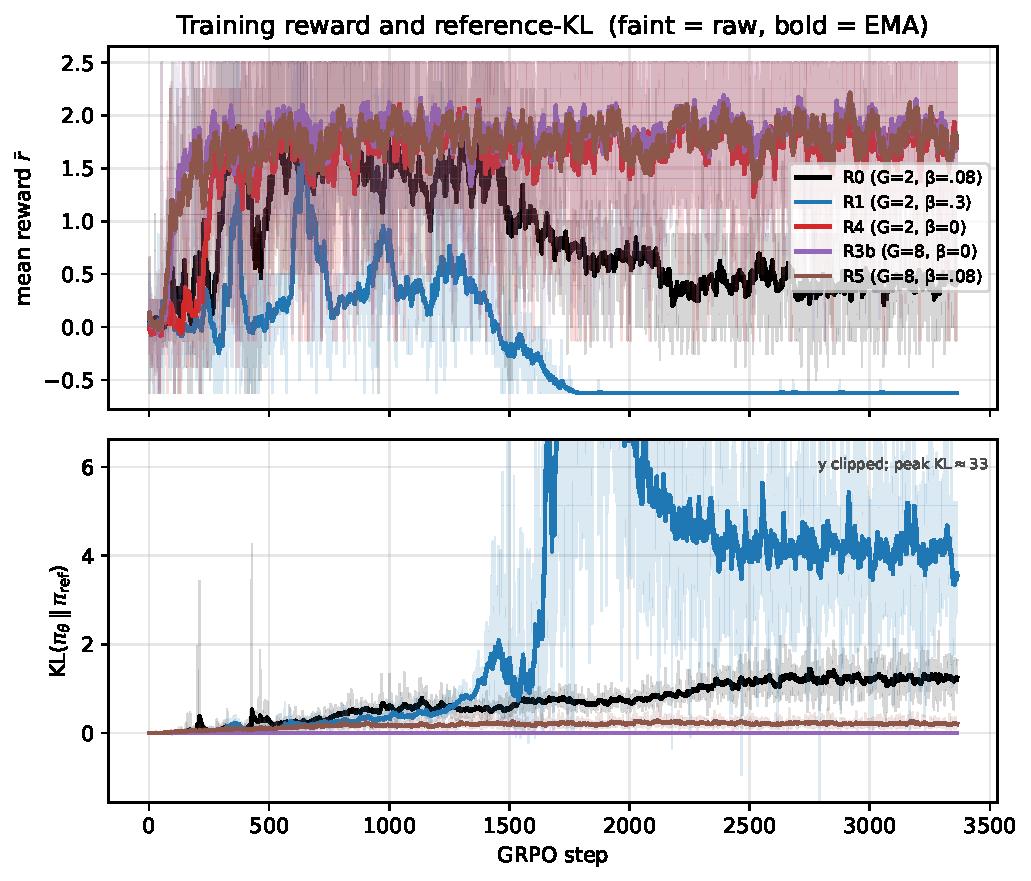
\includegraphics[width=0.58\linewidth]{F1_reward_kl.pdf}
\caption{Mean training reward $\bar r$ (top) and $\mathrm{KL}(\pi_\theta\Vert\pi_{\mathrm{ref}})$ (bottom) vs.\ GRPO step, for all five runs on shared axes. R0 over-optimises (reward peaks then declines) and R1 collapses (KL blow-up ${\sim}$step 1700); the $K{=}8$ runs (R3b, R5) and R4 stay stable.}
\label{fig:rewardkl}
\end{figure}

\begin{table}[t]
\centering\small
\caption{Held-out accuracy on the \emph{full} GSM8K test ($n{=}1319$, HF split, seed 42), greedy/exact-match, $\pm$95\% bootstrap CI; each run trained for the full \textbf{3364} GRPO steps (one epoch), scored at its \emph{best-val} (the saved checkpoint nearest the peak held-out validation \emph{reward}) and \emph{final} (step 3364) checkpoints.
Last column: \emph{paired} bootstrap $\Delta$ vs.\ base over the shared prompts (\code{paired\_ci.py}).
$\ast$ = paired 95\% CI excludes 0; $\dagger$ = collapse. The $\beta$-axis extension R1$(K{=}2,\beta{=}.3)$ fell \emph{below} base
(best 37.2 / final 0.0) --- a clean negative result.
All five runs are logged to the W\&B project \href{https://wandb.ai/sichengma0514-university-of-cambridge/a8-grpo}{\texttt{a8-grpo}}.}
\label{tab:acc}
\begin{tabular}{llrrr}
\toprule
Model & $(K,\beta)$, step & Acc.\,(\%) & 95\% CI & $\Delta$ base (paired) \\
\midrule
Base \code{gemma-3-1b-it} & --- & 47.4 & 44.7--50.0 & --- \\
R0 (baseline) & $(2,.08)$ best 700 & 46.7 & 44.0--49.4 & $-0.7$\ \,n.s. \\
R0 & $(2,.08)$ final 3364 & 6.2 & 4.9--7.5 & $-41.2^{\dagger}$ \\
R4 & $(2,0)$ best 1300 & 52.8 & 50.1--55.5 & $+5.4^{\ast}$ \\
R4 & $(2,0)$ final 3364 & 48.6 & 45.9--51.3 & $+1.2$\ \,n.s. \\
\textbf{R3b} & $(8,0)$ best 1000 & 55.7 & 53.0--58.2 & $+8.3^{\ast}$ \\
\textbf{R3b} & $(8,0)$ \textbf{final 3364} & \textbf{57.2} & 54.6--59.9 & $+9.9^{\ast}$ \\
R5 & $(8,.08)$ best 1300 & 53.4 & 50.7--56.2 & $+6.1^{\ast}$ \\
R5 & $(8,.08)$ final 3364 & 55.6 & 52.8--58.2 & $+8.2^{\ast}$ \\
\bottomrule
\end{tabular}
\end{table}

\textbf{(a) Accuracy} (Table~\ref{tab:acc}): base, the baseline R0, and the improved checkpoints on the full test ($n{=}1319$, seed 42), with
$\pm$95\% bootstrap and paired-$\Delta$ CIs over the shared prompts.

\textbf{(b) Training curves} (Fig.~\ref{fig:rewardkl}): mean reward and KL for the five runs on shared axes.

\textbf{(c) Diagnostic} (Fig.~\ref{fig:diag}): group degeneracy at $K{=}8$ --- about a third of groups are all-$K$-equal (zero advantage) yet
within-group $\sigma_r$ holds $\approx1.5$, not $\to0$.

\begin{figure}[H]
\centering
\begin{subfigure}{0.60\linewidth}\centering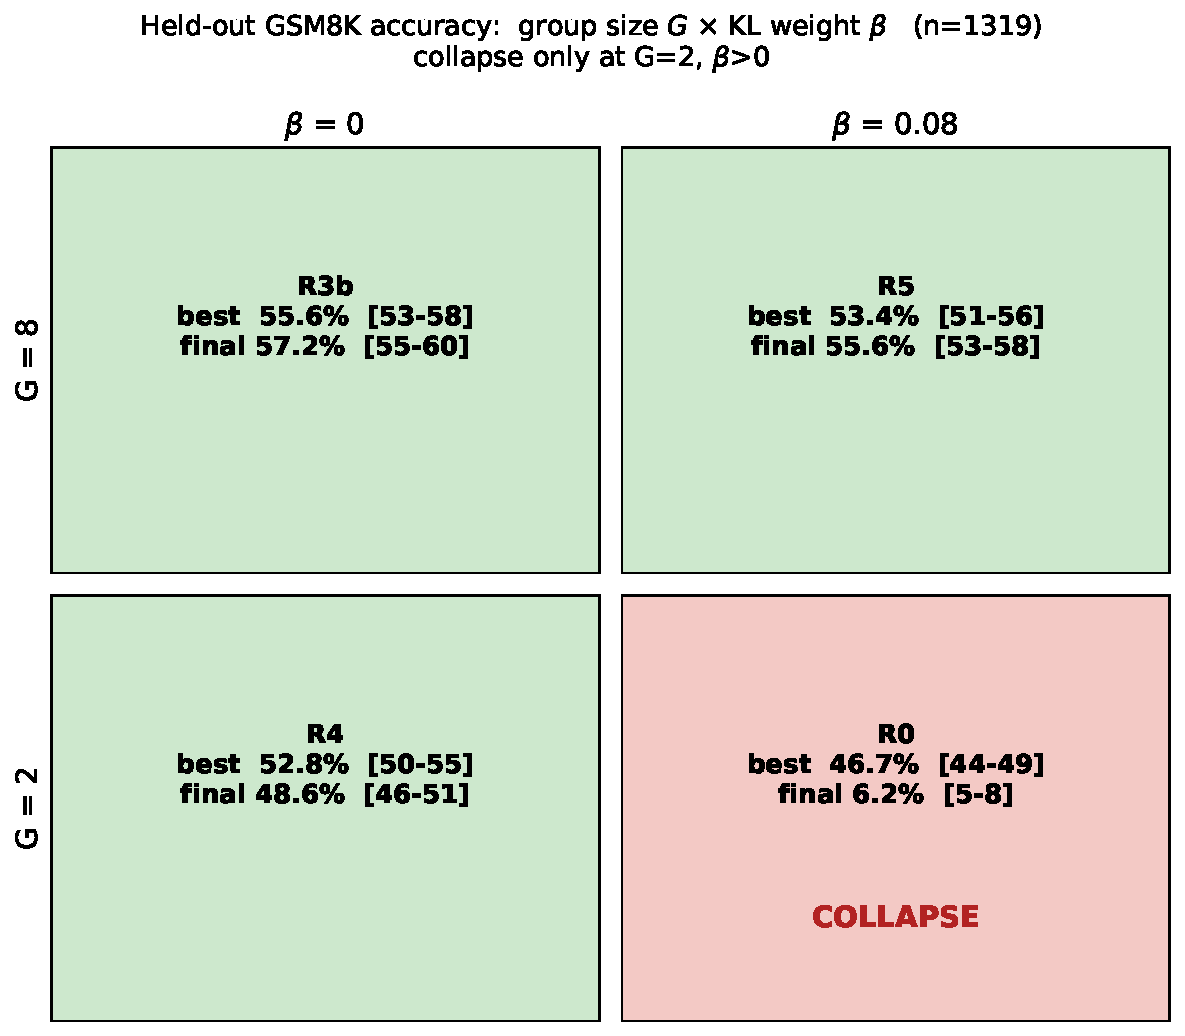
\includegraphics[width=\linewidth]{F4_2x2_GxB.pdf}\caption{$\beta\times K$ 2$\times$2 (best/final acc).}\label{fig:2x2}\end{subfigure}\hfill
\begin{subfigure}{0.60\linewidth}\centering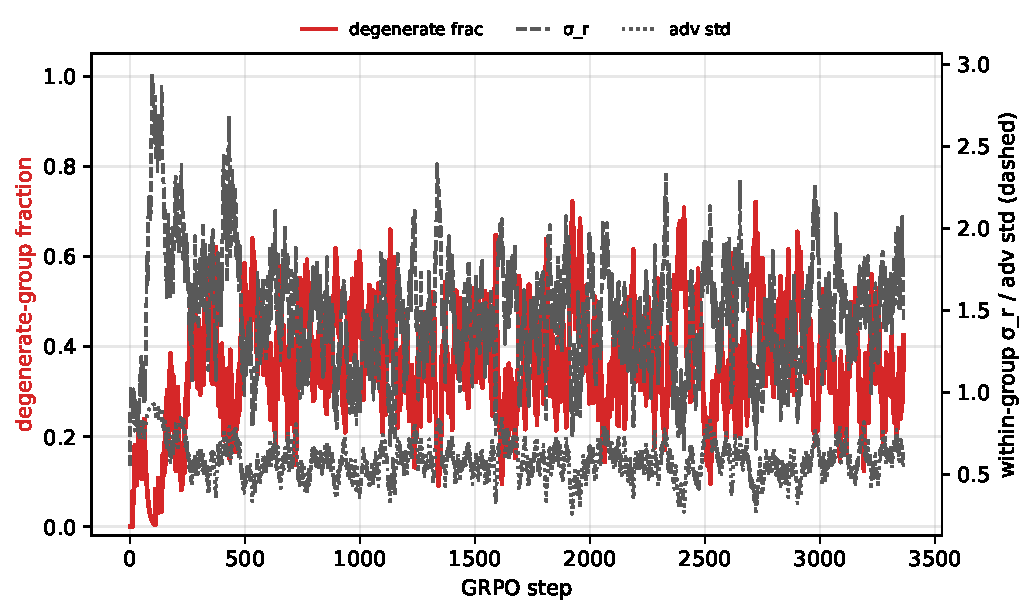
\includegraphics[width=\linewidth]{S3_group_degeneracy.pdf}\caption{Group degeneracy at $K{=}8$.}\label{fig:diag}\end{subfigure}
\caption{\emph{Left:} accuracy by $(K,\beta)$ --- collapse occurs \emph{only} at $K{=}2,\beta{>}0$ (R0). \emph{Right:} the diagnostic --- at $K{=}8$ about a
third of groups are degenerate (all-$K$ rewards equal) yet $\sigma_r$ holds $\approx1.5$ (steady, not $\to0$).}
\end{figure}

\textbf{(d) Findings vs.\ prediction.} \emph{Prediction (1) holds.} $K{=}8$ is the winning intervention: \textbf{R3b ($K{=}8,\beta{=}0$) is the best
model at 57.2\%} ($+9.9$\,pp over base, paired CI excludes 0); both $K{=}8$ runs beat base and each beats its matched $K{=}2$ run, and the 2$\times$2
(Fig.~\ref{fig:2x2}) shows over-optimisation is a $K{=}2$ phenomenon --- $K{=}2$ peaks then degrades (R4 $52.8\!\to\!48.6$; R0 collapses) while $K{=}8$
improves monotonically to the final step --- exactly as the lower $\operatorname{Var}(\hat g)$ predicts. \emph{Prediction (2) is contradicted.} The
tighter KL leash did not help: at $K{=}2$, $\beta{=}0$ (R4) beats $\beta{=}0.08$ (R0, which collapses) and pushing to $\beta{=}0.3$ (R1) collapsed
\emph{faster} (final 0\%); the collapse is confined to the $K{=}2,\beta{>}0$ corner, and at $K{=}8$ the KL weight is statistically irrelevant
(R3b vs.\ R5: $+1.7$\,pp, n.s.). The cure was variance reduction (group size), not regularisation --- echoing \axv{2503.14476}{DAPO}'s removal of the KL term for
long-output RL. The cost of $K{=}8$ is group degeneracy (Fig.~\ref{fig:diag}, the dead-group / effective-sample-size issue), but the net effect is
still $+8$--$10$\,pp.

\clearpage
\section*{I.4\quad GRPO theory --- written questions (40 marks)}

\subsection*{I.4.1 Group-mean normalisation}

Let $r_1,\dots,r_K$ be the group's i.i.d.\ rewards with mean $\mu$ and variance $\sigma^2$, $h_i$ the per-sample score, and $\hat A_i$ the std-normalised advantage; write
\[
\bar h=\frac{1}{K}\sum_{i=1}^K h_i.
\]

\paragraph{(i)}
Since $\mathbb{E}[r_i]=\mathbb{E}[\bar r]=\mu$,
\[
\mathbb{E}[\hat A_i]
=
\frac{\mathbb{E}[r_i-\bar r]}{\sigma}
=0.
\]
Because $X_i=h_i\hat A_i$ and $h_i$ is fixed, linearity of expectation gives
\[
\mathbb{E}[X_i]
=
h_i\,\mathbb{E}[\hat A_i]
=
h_i\cdot 0
=0,
\qquad
\mathbb{E}[X_i]=0.
\]
Summing over the group and again using linearity,
\[
\mathbb{E}[\hat g]
=
\mathbb{E}\!\left[\frac{1}{K}\sum_{i=1}^K X_i\right]
=
\frac{1}{K}\sum_{i=1}^K\mathbb{E}[X_i]
=
\frac{1}{K}\sum_{i=1}^K 0
=0,
\qquad
\mathbb{E}[\hat g]=0.
\]
Every expectation in this question is taken conditional on the sampled
responses $a_1,\dots,a_K$, which are held fixed; that is, $\mathbb{E}[\,\cdot\,]$
abbreviates $\mathbb{E}[\,\cdot\mid a_1,\dots,a_K]$, so each score $h_i$ is
constant and only the artificial reward noise is random. In the usual
policy-gradient problem the responses are sampled from the policy and their
rewards depend on the sampled responses, so the policy gradient need not vanish.

\paragraph{(ii)}
The common random term is the sample mean $\bar r$, appearing in every
\[
X_i=\frac{h_i}{\sigma}(r_i-\bar r).
\]
For $i\neq j$,
\begin{align*}
\operatorname{Cov}(r_i-\bar r,r_j-\bar r)
&=
\operatorname{Cov}(r_i,r_j)
-\operatorname{Cov}(r_i,\bar r)
-\operatorname{Cov}(\bar r,r_j)
+\operatorname{Var}(\bar r)\\
&=
0-\frac{\sigma^2}{K}-\frac{\sigma^2}{K}
+\frac{\sigma^2}{K}\\
&=
-\frac{\sigma^2}{K}.
\end{align*}
Hence
\[
\operatorname{Cov}(X_i,X_j)
=
-\frac{1}{K}h_i h_j^\top,
\qquad i\neq j.
\]
More precisely, the scalar covariance of the centred rewards is negative; the
cross-covariance matrix is a negative scalar multiple of $h_i h_j^\top$.
The negative dependence follows from the exact constraint
\[
\sum_{i=1}^K(r_i-\bar r)=0:
\]
if one centred reward increases, the others must collectively decrease.

\paragraph{(iii)}
The full covariance matrix is
\[
\operatorname{Cov}(\hat g)
=
\frac{1}{K^2}
\left[
\sum_{i=1}^K h_i h_i^\top
-
\frac{1}{K}
\left(\sum_{i=1}^K h_i\right)
\left(\sum_{j=1}^K h_j\right)^\top
\right]
=
\frac{1}{K^2}
\sum_{i=1}^K
(h_i-\bar h)(h_i-\bar h)^\top .
\]

For the scalar variance convention used in the lectures, define
\[
\operatorname{Var}_{\mathrm{tr}}(Z)
:=
\operatorname{tr}\!\left(\operatorname{Cov}(Z)\right).
\]
Taking the trace gives
\[
\operatorname{Var}_{\mathrm{tr}}(\hat g)
=
\frac{1}{K^2}
\sum_{i=1}^K
\|h_i-\bar h\|^2.
\]
Also,
\[
\operatorname{Cov}(X_1)
=
\left(1-\frac{1}{K}\right)h_1h_1^\top,
\]
and hence
\[
\operatorname{Var}_{\mathrm{tr}}(X_1)
=
\left(1-\frac{1}{K}\right)\|h_1\|^2.
\]
If one instead averaged $K$ independent copies of $X_1$, the naive i.i.d.
variance would be
\[
\operatorname{Var}_{\mathrm{tr,iid}}(\hat g)
=
\frac{1}{K}\operatorname{Var}_{\mathrm{tr}}(X_1).
\]

Following the lecture convention, define the effective sample size by
\[
\operatorname{Var}_{\mathrm{tr}}(\hat g)
=
\frac{\operatorname{Var}_{\mathrm{tr}}(X_1)}
{K_{\mathrm{eff}}}.
\]
Therefore
\[
K_{\mathrm{eff}}
=
\frac{
\operatorname{Var}_{\mathrm{tr}}(X_1)
}{
\operatorname{Var}_{\mathrm{tr}}(\hat g)
}
=
\frac{
K^2\left(1-\frac{1}{K}\right)\|h_1\|^2
}{
\sum_{i=1}^K\|h_i-\bar h\|^2
}
=
\frac{
K(K-1)\|h_1\|^2
}{
\sum_{i=1}^K\|h_i-\bar h\|^2
}.
\]
Equivalently, its discrepancy from the nominal sample size $K$ is
\[
\frac{K_{\mathrm{eff}}}{K}
=
\frac{
\operatorname{Var}_{\mathrm{tr,iid}}(\hat g)
}{
\operatorname{Var}_{\mathrm{tr}}(\hat g)
}.
\]

If
\[
\frac{1}{K}\sum_{i=1}^K\|h_i-\bar h\|^2
\]
remains of constant order and $\|h_1\|^2=O(1)$, then
\[
K_{\mathrm{eff}}=\Theta(K)
\]
as $K\to\infty$.

If all score vectors lie in one direction, write
\[
h_i=c_i v.
\]
Then
\[
\operatorname{Cov}(\hat g)
=
\frac{vv^\top}{K^2}
\sum_{i=1}^K(c_i-\bar c)^2,
\]
so the covariance has rank at most one, and
\[
K_{\mathrm{eff}}
=
\frac{
K(K-1)c_1^2
}{
\sum_{i=1}^K(c_i-\bar c)^2
}.
\]
Thus only variation in the scalar coefficients $c_i$ contributes to the
variance. In the special case $h_i=h$ for every $i$,
\[
\hat g
=
\frac{h}{K}\sum_{i=1}^K\hat A_i
=0
\]
for every reward realisation. Hence
$\operatorname{Cov}(\hat g)=0$ and, provided $h\neq0$, the effective sample size
is formally infinite.


\subsection*{I.4.2 KL-regularised policy update}

\paragraph{(i)}
With step size $\eta>0$ (the inverse weight on the KL proximal term), the objective is
\[
F(\pi)
=
\sum_a\pi(a)A_t(a)
-\frac{1}{\eta}
\sum_a\pi(a)\log\frac{\pi(a)}{\pi_t(a)}.
\]
Introducing a Lagrange multiplier $\lambda$ for $\sum_a\pi(a)=1$, stationarity
on the support of $\pi_t$ gives
\[
A_t(a)
-\frac{1}{\eta}
\left(
\log\frac{\pi(a)}{\pi_t(a)}+1
\right)
+\lambda=0.
\]
Consequently,
\[
\pi_{t+1}(a)
=
\frac{\pi_t(a)\exp(\eta A_t(a))}
{\sum_b\pi_t(b)\exp(\eta A_t(b))}.
\]
Actions outside the support of $\pi_t$ remain assigned zero probability. The
objective is strictly concave on this support, so the optimiser is unique,
assuming the normalising constant is finite.

For small $\eta$, expanding $\exp(\eta A_t)=1+\eta A_t+O(\eta^2)$ in both the numerator and the denominator and keeping first order,
\[
\pi_{t+1}(a)
=
\pi_t(a)
\left[
1+\eta\left(A_t(a)-\mathbb{E}_{\pi_t}[A_t]\right)
\right]
+O(\eta^2),
\]
so $\eta$ controls the update size: large $\eta$ places increasingly more mass on high-advantage actions.

\paragraph{(ii)}
For the true advantage of $\pi_t$,
\[
J(\pi_t)
=
\mathbb{E}_{a\sim\pi_t}[A^{\pi_t}(a)]
=0.
\]
The regularised objective evaluated at $\pi_t$ is also zero. Since
$\pi_{t+1}$ maximises it,
\[
J(\pi_{t+1})
-\frac{1}{\eta}
\operatorname{KL}(\pi_{t+1}\Vert\pi_t)
\geq 0.
\]
It follows that
\[
J(\pi_{t+1})
\geq
\frac{1}{\eta}
\operatorname{KL}(\pi_{t+1}\Vert\pi_t)
\geq 0
=
J(\pi_t).
\]
Thus the update guarantees monotone improvement in the scalar performance
measure defined in the question.

In neural-network GRPO the guarantee may fail because the exact advantage is
replaced by a noisy finite-sample estimate and the maximisation is replaced by
a finite number of stochastic-gradient steps in a restricted parametric policy
class. The clipped GRPO objective is also not identical to the exact
KL-regularised objective above.

\paragraph{(iii)}
For one sample, write
\[
\ell(\rho,\hat A)
=
\min\left(
\rho\hat A,
\operatorname{clip}(\rho,1-\epsilon,1+\epsilon)\hat A
\right).
\]
Equivalently,
\[
\ell(\rho,\hat A)
=
\begin{cases}
\hat A\min(\rho,1+\epsilon), & \hat A\geq 0,\\[2mm]
\hat A\max(\rho,1-\epsilon), & \hat A<0.
\end{cases}
\]
Thus, for a positive advantage, the objective gives no further incentive to
increase the ratio above $1+\epsilon$. For a negative advantage, it gives no
further incentive to reduce the ratio below $1-\epsilon$.

This is not a hard constraint
\[
\rho\in[1-\epsilon,1+\epsilon].
\]
Other samples can still move the ratio outside this interval. In contrast, a
constraint
\[
\operatorname{KL}
\bigl(
\pi_\theta(\cdot\mid q)
\Vert
\pi_{\mathrm{old}}(\cdot\mid q)
\bigr)
\leq\delta
\]
is a constraint on the whole distribution $\pi_\theta(\cdot\mid q)$. Although this
is a single distribution over the action, the divergence
$\sum_a\pi_\theta(a\mid q)\log\frac{\pi_\theta(a\mid q)}{\pi_{\mathrm{old}}(a\mid q)}$
depends on the probabilities of all actions simultaneously, including unsampled
ones. PPO clipping, by contrast, acts only on the ratio at each individual
sampled action and is advantage-dependent; it does not directly constrain
unsampled actions, and does not guarantee that this distribution-level KL
divergence is small.


\subsection*{I.4.3 Mixture proposal and importance weighting}

We suppress the fixed prompt $q$ from the notation. Define
\[
    p(a) := \pi_{\mathrm{old}}(a\mid q),
    \qquad
    u(a) := \pi_{\mathrm{unif}}(a\mid q),
    \qquad
    m_\alpha(a) := \pi_{\mathrm{mix}}(a\mid q)
    = (1-\alpha)p(a)+\alpha u(a),
\]
and
\[
    s_\theta(a):=\nabla_\theta \log \pi_\theta(a\mid q).
\]
Here $\alpha\in(0,1)$ is the mixing weight (the fraction of uniform exploration $u$ blended into $p$). Assume $m_\alpha(a)>0$ whenever $p(a)>0$.

\paragraph{(i)}
The true policy gradient is an expectation under $p=\pi_{\mathrm{old}}$. Importance sampling rewrites any such expectation as one
under $m_\alpha=\pi_{\mathrm{mix}}$, namely $\E_{a\sim p}[F]=\E_{a\sim m_\alpha}[w(a)\,F]$ with weight $w(a)=p(a)/m_\alpha(a)$;
drawing $a_i\overset{\mathrm{iid}}{\sim}\pi_{\mathrm{mix}}$ therefore gives the estimator and its explicit weight
\[
    \widehat g_{\mathrm{mix}}=\frac1K\sum_{i=1}^K w_i\,s_\theta(a_i)\,\widehat A_i,
    \qquad
    w_i=\frac{\pi_{\mathrm{old}}(a_i\mid q)}{(1-\alpha)\,\pi_{\mathrm{old}}(a_i\mid q)+\alpha\,\pi_{\mathrm{unif}}(a_i\mid q)}.
\]
The weight corrects the sampling distribution from $m_\alpha$ back to $p$; the correct empirical advantage $\widehat A_i$ is addressed in (iii).

\paragraph{(ii)}
For every fixed realised action $a_i$,
\[
    m_\alpha(a_i)\to p(a_i),
    \qquad
    w_i=\frac{p(a_i)}{m_\alpha(a_i)}\to1.
\]
Therefore
\[
    \widehat g_{\mathrm{mix}}
    \to
    \frac1K\sum_{i=1}^K s_\theta(a_i)\widehat A_i.
\]
With the standard GRPO empirical advantage
\[
    \widehat A_i=\frac{r_i-\bar r}{\sigma_r},
\]
we obtain
\[
    \widehat g_{\mathrm{mix}}\to \widehat g_{\mathrm{GRPO}}.
\]
The same statement holds if a weighted mean and weighted standard deviation are used, since $w_i\to1$ implies that the weighted empirical statistics converge to the ordinary ones for the same realised actions.

\paragraph{(iii-a)}
Let
\[
    \mu_p:=V^{\pi_{\mathrm{old}}}(q),
    \qquad
    \mu_u:=V^{\pi_{\mathrm{unif}}}(q),
    \qquad
    \mu_m:=V^{\pi_{\mathrm{mix}}}(q).
\]
Then, by linearity of expectation,
\[
\begin{aligned}
    V^{\pi_{\mathrm{mix}}}(q)
    &=
    \sum_a \bigl((1-\alpha)p(a)+\alpha u(a)\bigr)R(q,a) \\
    &=
    (1-\alpha)V^{\pi_{\mathrm{old}}}(q)
    +
    \alpha V^{\pi_{\mathrm{unif}}}(q).
\end{aligned}
\]
Hence
\[
    V^{\pi_{\mathrm{mix}}}(q)
    =
    (1-\alpha)V^{\pi_{\mathrm{old}}}(q)
    +
    \alpha V^{\pi_{\mathrm{unif}}}(q).
\]

\paragraph{(iii-b)}
No. The importance weight $w_i$ re-targets the sampling distribution from $m_\alpha$ back to $p$, but the baseline is still the unweighted group mean $\bar r$, which under mixture sampling estimates $\mu_m=V^{\pi_{\mathrm{mix}}}(q)$, not $\mu_p=V^{\pi_{\mathrm{old}}}(q)$. Centring with this wrong baseline and applying only the outer weight gives
\[
    \E_m\!\left[w\,s_\theta\,(R-\mu_m)\right]
    =
    \E_p\!\left[s_\theta\,(R-\mu_p)\right]
    +(\mu_p-\mu_m)\,\E_p[s_\theta],
\]
whose first term is the target $\pi_{\mathrm{old}}$ gradient and where $\mu_p-\mu_m=\alpha(\mu_p-\mu_u)$. The residual $(\mu_p-\mu_m)\,\E_p[s_\theta]$ vanishes only when $\E_p[s_\theta]=0$, which the score identity gives exactly at $\theta=\theta_{\mathrm{old}}$ (where $p=\pi_\theta$) but not after any update step. So $w$ alone is enough only at $\theta=\theta_{\mathrm{old}}$; in general the baseline must be re-estimated under $p$.

Using the same weights, the old-policy baseline can be estimated by
\[
    \widehat\mu_p^{\mathrm{IS}}=\frac1K\sum_{j=1}^K w_jr_j
    \qquad\text{or}\qquad
    \widehat\mu_p^{\mathrm{SN}}=\frac{\sum_{j=1}^K w_jr_j}{\sum_{j=1}^K w_j}.
\]
The IS form is unbiased, since the weight undoes the change of sampling law:
\[
\begin{aligned}
    \E\!\left[\widehat\mu_p^{\mathrm{IS}}\right]
    &=\E_m[wR]
    =\sum_a m_\alpha(a)\,\frac{p(a)}{m_\alpha(a)}\,R(q,a)\\
    &=\sum_a p(a)\,R(q,a)=\mu_p,
\end{aligned}
\]
while $\widehat\mu_p^{\mathrm{SN}}$ is consistent ($\E_m[w]=1$) but slightly biased at finite $K$. With the analogously weighted $\widehat\sigma_p$, the reweighted advantage that keeps $\widehat g_{\mathrm{mix}}$ unbiased for the $\pi_{\mathrm{old}}$ gradient is then
\[
    \widetilde A_i=w_i\frac{r_i-\widehat\mu_p}{\widehat\sigma_p},
    \qquad
    \widehat g_{\mathrm{mix}}=\frac1K\sum_{i=1}^K s_\theta(a_i)\,\widetilde A_i.
\]

\paragraph{(iv)}
Let
\[
    A_p(a):=R(q,a)-\mu_p,
    \qquad
    Z(a):=s_\theta(a)A_p(a),
    \qquad
    g:=\E_p[Z(a)].
\]
Ignoring empirical baseline and variance estimation, the old-policy estimator has covariance
\[
    \Cov(\widehat g_{\mathrm{GRPO}})
    =
    \frac1K\left(\E_p[ZZ^\top]-gg^\top\right).
\]
The importance-sampled estimator has covariance
\[
\begin{aligned}
    \Cov(\widehat g_{\mathrm{mix}})
    &=
    \frac1K\left(\E_m[w^2ZZ^\top]-gg^\top\right) \\
    &=
    \frac1K\left(\E_p[wZZ^\top]-gg^\top\right).
\end{aligned}
\]
Therefore
\[
    \Cov(\widehat g_{\mathrm{mix}})
    -
    \Cov(\widehat g_{\mathrm{GRPO}})
    =
    \frac1K\E_p[(w-1)ZZ^\top].
\]
There is no universal ordering: importance sampling can either increase or decrease variance.

For the scalar advantage contribution alone,
\[
    \Var_m(wA_p)-\Var_p(A_p)
    =
    \E_p[(w-1)A_p^2].
\]
For $\alpha>0$,
\[
    w(a)>1
    \iff
    m_\alpha(a)<p(a)
    \iff
    u(a)<p(a),
\]
and
\[
    w(a)<1
    \iff
    m_\alpha(a)>p(a)
    \iff
    u(a)>p(a).
\]

Therefore, if large-magnitude advantages occur mainly on actions satisfying $u(a)<p(a)$, then $w(a)>1$ where $A_p(a)^2$ is large, so
\[
    \E_p[(w-1)A_p^2]>0,
\]
and the variance increases.

Conversely, if large-magnitude advantages occur mainly on actions satisfying $u(a)>p(a)$, then $w(a)<1$ where $A_p(a)^2$ is large, so
\[
    \E_p[(w-1)A_p^2]<0,
\]
and the variance decreases.

\paragraph{(v-a)}
Since $0<c<1$ we have $\log c<0$, so
\[
    \,w_i=c^T=e^{T\log c}\longrightarrow 0\ \text{ exponentially fast as }T\to\infty.\,
\]
A value $c<1$ is the typical situation when $\alpha>0$ because the responses are drawn from $\pi_{\mathrm{mix}}$, whose uniform component inflates the probability of tokens that are unlikely under $\pi_{\mathrm{old}}$, so the sampled tokens usually satisfy $\pi_{\mathrm{mix}}>\pi_{\mathrm{old}}$, i.e.\ $c=\pi_{\mathrm{old}}/\pi_{\mathrm{mix}}<1$.

\paragraph{(v-b)}
When $w_i=c^T$ is exponentially small, almost every sampled trajectory contributes negligible gradient signal, so $\widehat g_{\mathrm{mix}}$ is dominated by a handful of rare large-weight trajectories: the effective sample size collapses and the variance explodes, making the estimate unreliable for long responses.

One concrete fix is to shrink the mixture weight with length, taking $\alpha=\alpha_T=O(1/T)$ so that the per-token ratio satisfies $c_T=1-\kappa/T+o(1/T)$ and the full-response weight stays bounded away from zero,
\[
    w_i=c_T^{\,T}\longrightarrow e^{-\kappa}>0 .
\]
The trade-off is weaker uniform exploration on long responses.

\clearpage
\partheading{Part II --- Adaptive planning in \texttt{cmbagent\_lg}}

\noindent Studied in full at commit \href{https://github.com/borisbolliet/cmbagent_lg/tree/d7d0592a714e4cc01c97f1b77afdd57a208b18db}{\texttt{d7d0592}}
(\texttt{adaptive-planning} branch), module \href{https://github.com/borisbolliet/cmbagent_lg/tree/d7d0592a714e4cc01c97f1b77afdd57a208b18db/cmbagent_lg/adaptive_planning}{\texttt{cmbagent\_lg/adaptive\_planning}}
(graph, nodes, state, schemas, prompts), which composes the \texttt{planning/} and \texttt{deep\_research/} modules.

\section*{II.1\quad Workflow diagram}

\begin{figure}[h]
\centering
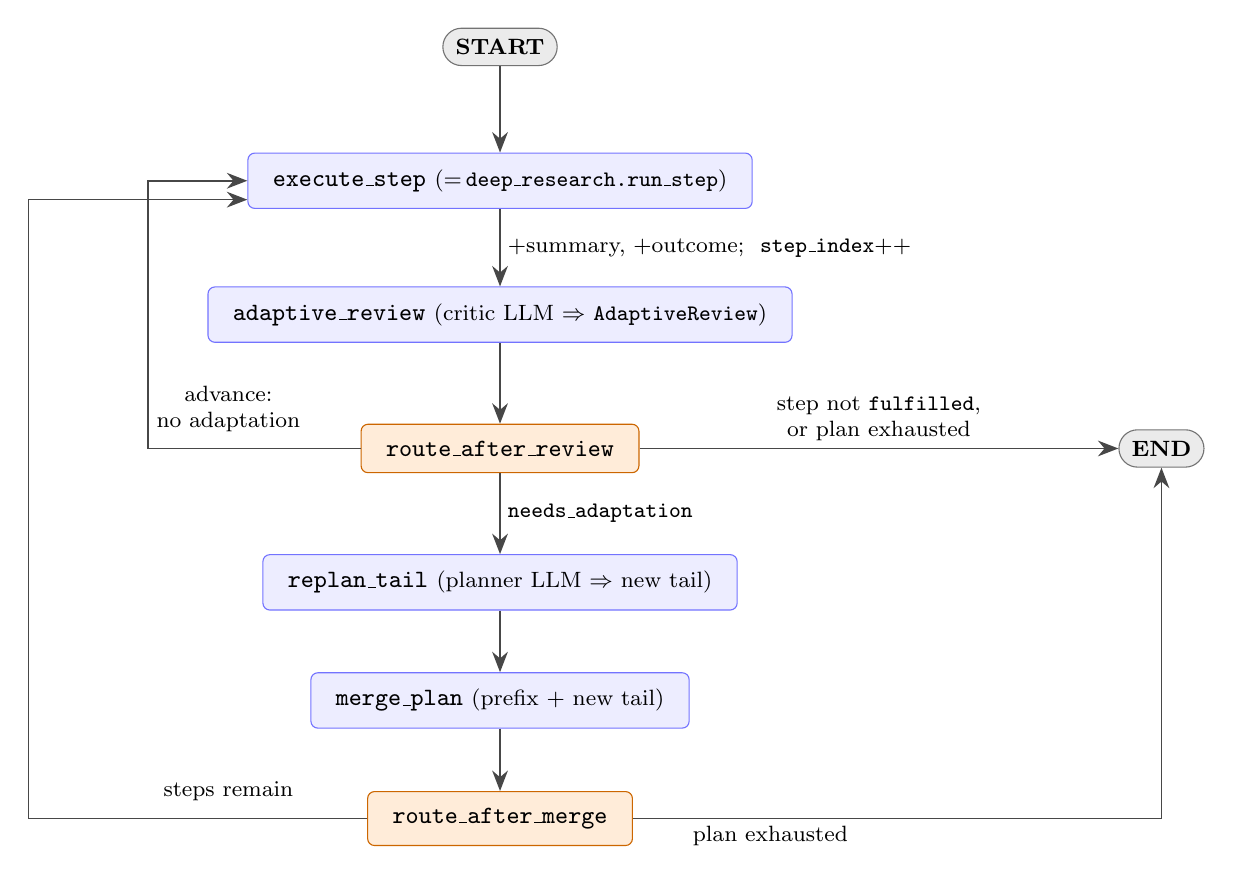
\begin{tikzpicture}[
  >={Stealth[length=2.6mm,width=2mm]}, font=\small,
  proc/.style={rectangle, rounded corners=2.5pt, draw=blue!55, fill=blue!7, align=center,
               inner xsep=9pt, inner ysep=6pt},
  rt/.style={rectangle, rounded corners=2.5pt, draw=orange!80!black, fill=orange!15, align=center,
             inner xsep=9pt, inner ysep=6pt},
  term/.style={rounded rectangle, draw=black!55, fill=black!8, align=center, inner sep=4pt, font=\footnotesize\bfseries},
  e/.style={->, semithick, draw=black!72},
  lbl/.style={font=\footnotesize, inner sep=2.5pt, fill=white},
]
\node[term] (start) at (0,0) {START};
\node[proc] (exec)   at (0,-1.7) {\code{execute\_step} {\footnotesize($=$\,\code{deep\_research.run\_step})}};
\node[proc] (rev)    at (0,-3.4) {\code{adaptive\_review} {\footnotesize(critic LLM $\Rightarrow$ \code{AdaptiveReview})}};
\node[rt]   (r1)     at (0,-5.1) {\code{route\_after\_review}};
\node[proc] (replan) at (0,-6.8) {\code{replan\_tail} {\footnotesize(planner LLM $\Rightarrow$ new tail)}};
\node[proc] (merge)  at (0,-8.3) {\code{merge\_plan} {\footnotesize(prefix $+$ new tail)}};
\node[rt]   (r2)     at (0,-9.8) {\code{route\_after\_merge}};
\node[term] (end)    at (8.4,-5.1) {END};

\draw[e] (start) -- (exec);
\draw[e] (exec)  -- (rev)  node[lbl,midway,right]{$+$summary, $+$outcome;\ \ \code{step\_index}{+}{+}};
\draw[e] (rev)   -- (r1);
\draw[e] (r1)    -- (replan) node[lbl,midway,right]{\code{needs\_adaptation}};
\draw[e] (replan)-- (merge);
\draw[e] (merge) -- (r2);
\draw[e] (r1.east) -- (end.west) node[lbl,midway,above,align=center]{step not \code{fulfilled},\\ or plan exhausted};
\draw[e] (r2.east) -| (end) node[lbl,pos=0.13,below]{plan exhausted};
% back-edges to execute_step (next step)
\draw[e] (r1.west) -- ++(-2.7,0) |- (exec.west);
\draw[e] (r2.west) -- ++(-4.3,0) |- ([yshift=-2.4mm]exec.west);
\node[lbl,align=center] at (-3.45,-4.6) {advance:\\ no adaptation};
\node[lbl] at (-3.45,-9.45) {steps remain};
\end{tikzpicture}
\caption{Adaptive-planning LangGraph graph (\code{adaptive\_planning/graph.py}). Blue $=$ work nodes, orange $=$ conditional
routers; the threaded \code{AdaptivePlanState} carries \code{plan}, \code{step\_index}, \code{step\_summaries}/\code{step\_outcomes},
\code{adaptive\_review}, \code{new\_tail}, \code{adaptive\_history}. \emph{(Excluded from the 2-page limit.)}}
\end{figure}

\noindent\textbf{Walkthrough.} The initial \code{Plan} comes from the bounded propose--critique loop in \code{planning/}; this graph
executes it. \code{execute\_step} (\code{deep\_research}'s \code{run\_step}, reused verbatim) runs the step at \code{step\_index},
appends a summary and a structured outcome \{\code{fulfilled},\dots\}, increments \code{step\_index}, and always passes to
\code{adaptive\_review}. The four things the brief asks for:
\begin{itemize}[leftmargin=2.2em,label={},topsep=3pt,itemsep=4pt]
\item \textbf{What triggers a revision:} \code{adaptive\_review} --- a critic LLM given the overall task, the latest step's
summary$+$outcome, and the unrun steps --- returns \code{AdaptiveReview(needs\_adaptation, recommendations)}.
\code{route\_after\_review} branches to \code{replan\_tail} \emph{iff} the step was \code{fulfilled}, the plan is not exhausted,
\emph{and} \code{needs\_adaptation} is set; otherwise it advances to the next step or halts at \code{END}.
\item \textbf{What may change:} only the \emph{tail} \code{plan.sub\_tasks[n\_done:]}: \code{replan\_tail} asks the planner LLM (given the
completed summaries, the current tail, and the recommendations) for a replacement tail, and \code{merge\_plan} sets
\code{plan = completed\_prefix + new\_tail}.
\item \textbf{What is held fixed:} the completed prefix \code{plan.sub\_tasks[:n\_done]}, its stored summaries/outcomes, and
\code{step\_index} are never touched by a revision, so executed work is neither re-run nor re-ordered.
\item \textbf{How it terminates:} a router returns \code{END} as soon as a step is \emph{not} \code{fulfilled} or the plan is exhausted
(\code{step\_index $>$ len(plan)}); \code{execute\_step} advances \code{step\_index} by one per step while a revision never does, so
the plan is consumed only by execution and the loop halts once the replanner stops extending the tail. The sole hard backstop is
LangGraph's default \code{recursion\_limit}, which \emph{raises} rather than finishing --- whether this is a genuine guarantee is
taken up in II.2.
\end{itemize}

\section*{II.2\quad Problems}

\textbf{P1 --- Termination is not \emph{guaranteed}.} The graph \emph{does} have a stopping rule --- \code{route\_after\_review}
and \code{route\_after\_merge} return \code{END} the moment a step is not \code{fulfilled} or the plan is exhausted
(\code{step\_index $>$ len(plan)}), so a well-behaved run does terminate. The defect is that nothing \emph{forces} that rule to be
reached: \code{step\_index} advances only in \code{execute\_step}, whereas \code{replan\_tail} may return a tail \emph{longer} than
the steps it replaces and \code{merge\_plan} routes straight back into execution. With no revision budget, no length cap and no
monotone quantity that must strictly decrease, the plan can grow without bound and the ``exhausted'' condition recede forever.
Closed-loop control is well-behaved only when the feedback law contracts toward the goal (a Lyapunov/termination argument), and a
free-text ``keep the tail minimal'' instruction to an LLM is no such contraction. The only hard backstop, \code{recursion\_limit},
surfaces as an \emph{exception}, not a finished run --- and the bounded-loop safeguard the initial planner relies on
(\code{num\_rounds}) was dropped here.

\textbf{P2 --- Adaptation is scoped to successful steps, not to recovery.} The loop revises only after a \emph{successful} step:
\code{route\_after\_review} tests \code{fulfilled} \emph{before} \code{needs\_adaptation}, so a \code{fulfilled=False} outcome routes
to \code{END} (the \code{adaptive\_review} verdict, though computed, then goes unused). This is a coherent design --- adaptation here
is meant to make an \emph{already-working} execution more responsive to what it has learned, not to repair a failing one. The
limitation is that the closed-loop benefit (using feedback to correct course) stays confined to the success path: a failed step
simply ends the run, with no retry or route-around. Where a failed step is often recoverable, extending adaptation to that case
(II.3) would widen the benefit.

\textbf{P3 --- The replanned tail bypasses the reviewer that gates the initial plan.} \code{planning/} accepts a plan only after a
bounded \code{planner}$\leftrightarrow$\code{plan\_reviewer} propose--critique loop. The adaptive replan has \emph{no} reviewer:
\code{merge\_plan} splices the planner's \code{new\_tail} unchecked. Revisions --- generated mid-run under the pressure of a
surprising result, i.e.\ exactly when error is likeliest --- thus receive \emph{weaker} quality control than the original plan, and
can drift from \code{main\_task} or contradict the frozen prefix with nothing to catch it.

\textbf{P4 --- Partial-state feedback at unconditional cost.} \code{adaptive\_review} sees only the \emph{last} step's summary$+$outcome and
the remaining steps --- not the full trajectory or the artifacts produced --- so its decision is conditioned on the last step alone (effectively Markov)
and cross-step drift is invisible; closed-loop control needs full-state feedback, not a single observation. It also fires after
\emph{every} step regardless of need (and the planner on every revision), so token cost and latency scale with plan length with no
gating.

\section*{II.3\quad Proposed improvements}

\textbf{P1 $\to$ bound the loop.} Thread a \code{revision\_budget} (and/or \code{max\_steps}) through \code{AdaptivePlanState},
decrement it in \code{merge\_plan}, and have the routers \emph{finish gracefully} (run out the current tail, then \code{END}) once it
hits zero; optionally reject any \code{new\_tail} that would push the plan past a length cap. \emph{Why:} reinstates a
strictly-decreasing quantity, so termination no longer rests on LLM goodwill. \emph{Trade-off:} a hard cap can truncate a genuinely
expanding task --- so surface ``budget exhausted'' as an explicit, inspectable outcome rather than a silent stop.

\textbf{P2 $\to$ add a recovery path on failure.} On \code{fulfilled=False}, route to \code{replan\_tail} (or a dedicated
\code{repair} node) with a per-step retry budget, halting only after $K$ failed attempts. \emph{Why:} extends the closed-loop
benefit to the failure case --- a recoverable error drives a re-plan rather than ending the run.
\emph{Trade-off:} extra execution/LLM cost and a risk of looping on an impossible step, both bounded by the retry budget; needs a
recoverable-vs-fatal flag in the outcome.

\textbf{P3 $\to$ validate the replanned tail.} Before \code{merge\_plan}, pass \code{new\_tail} through the existing \code{planning}
\code{plan\_reviewer} for one critique round against \code{main\_task} and the frozen prefix, regenerating if it diverges.
\emph{Why:} gives revisions the same quality gate as the initial plan, closing the asymmetry in P3. \emph{Trade-off:} one extra
reviewer call (and possibly a planner re-pass) per revision --- bound it to a single round to cap added latency.

\textbf{P4 $\to$ richer, gated feedback.} Give the reviewer the full step history and original goal (global state), and \emph{gate}
the call --- use a cheap model (or skip it) when the outcome shows no downstream impact, escalating to the full critic only on
flagged steps. \emph{Why:} full-state feedback catches multi-step drift; gating removes the per-step tax. \emph{Trade-off:} more
context costs tokens, and gating risks missing a non-obvious adaptation --- so gate conservatively.

\end{document}
